\documentclass[border=10pt]{standalone}

\usepackage{tikz}
\usepackage{tikzsymbols}
\usetikzlibrary{calc,patterns,shapes.geometric}

\def\centerarc[#1](#2)(#3:#4:#5){\draw[#1] ($(#2)+({#5*cos(#3)},{#5*sin(#3)})$) arc (#3:#4:#5);}

\begin{document}
	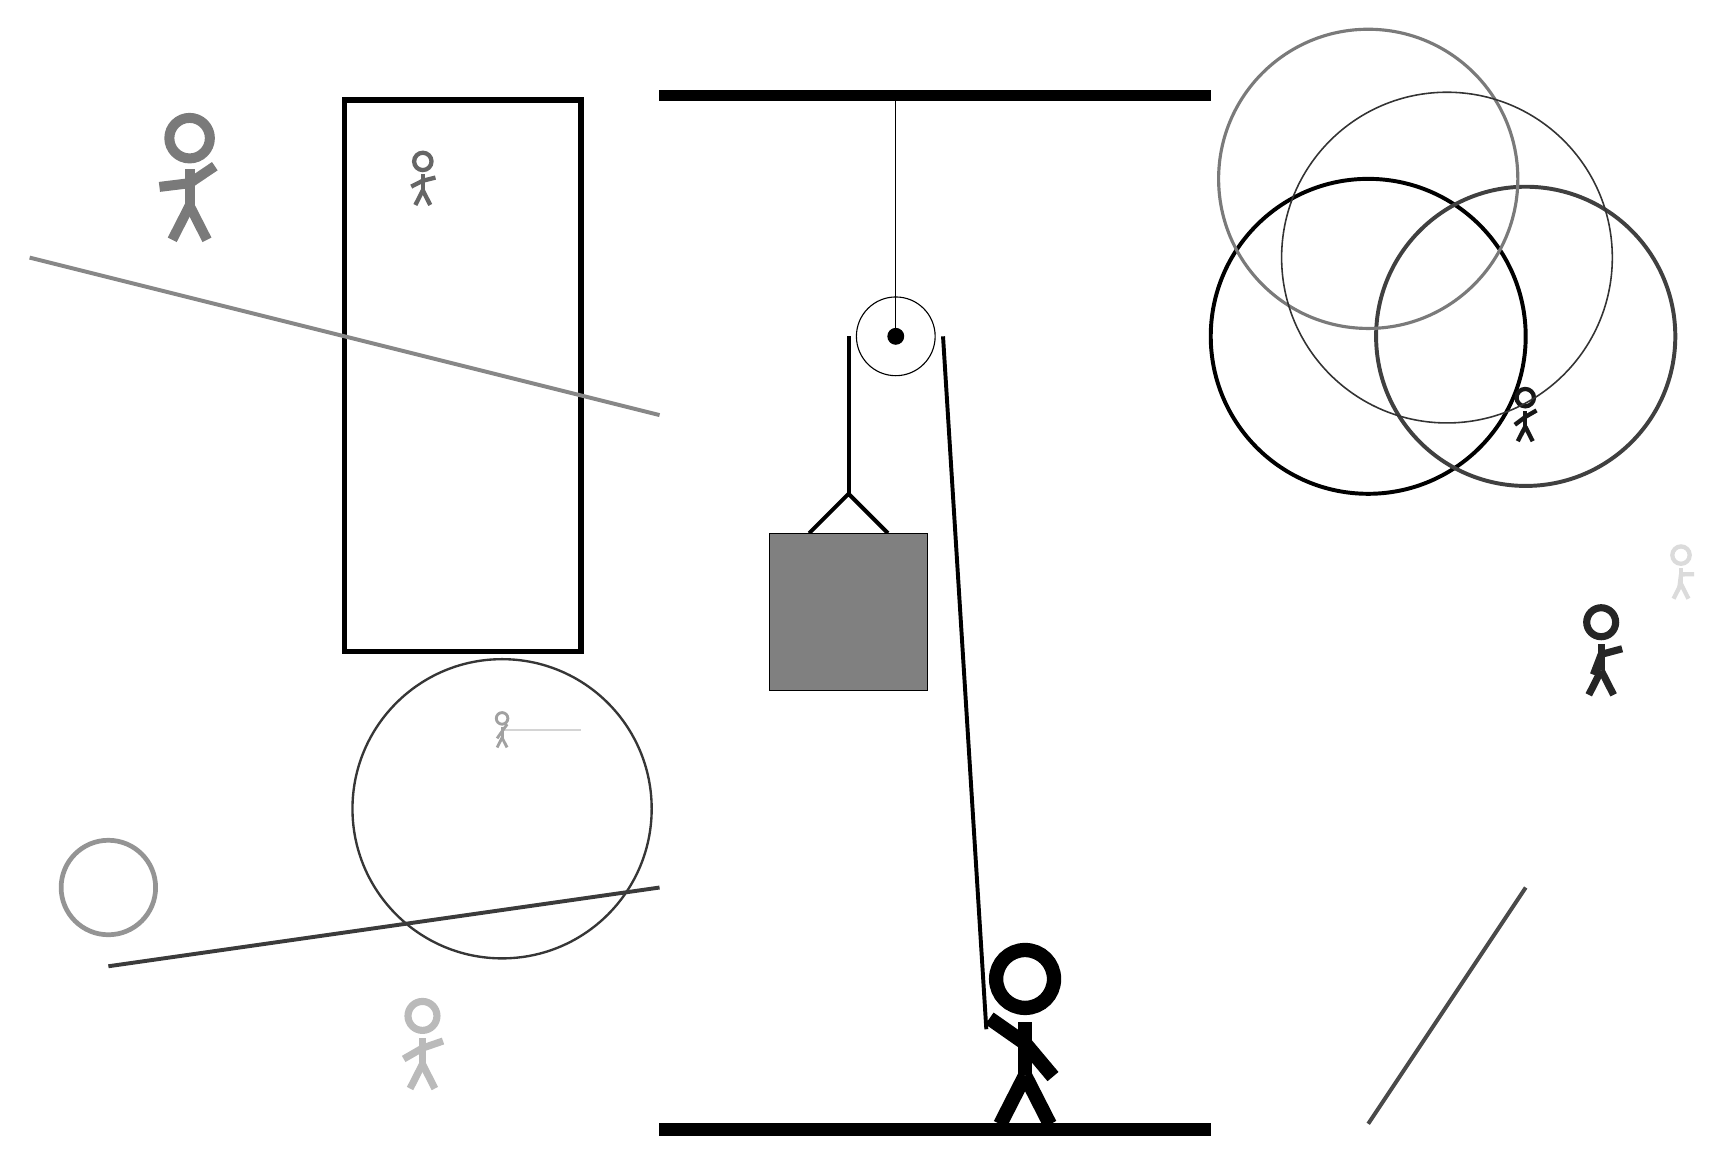
\begin{tikzpicture}
		%%%%% START %%%%%
		
		\draw[fill=black] (-2, 10) rectangle (5, 10.125);
		
		\draw (1, 7) circle (0.5);
		\draw[fill=black] (1, 7) circle (0.1);
		\draw (1, 10) -- (1, 7);
		
		\draw[line width=0.5mm] (-0.1, 4.5) -- (0.4, 5.0) -- (0.9, 4.5);
		\draw[fill=black!50] (-0.6, 4.5) rectangle (1.4, 2.5);
		
		\draw[line width=0.5mm] (0.4, 7) -- (0.4, 5.0);
		\centerarc[line width=0.5mm](1, 7)(0:180:0.6);
		\draw[line width=0.5mm](1.6, 7) -- (2.15, -1.8);
		
		\node at (2.6, -1.9) {\Strichmaxerl[10][-35][-50]};
		
		\node[line width=0.5mm, color=black!14] at (11, 4) {\Strichmaxerl[3][83][1]};
		
		\draw [line width=0.3mm, color=black!79](-4, 1) circle (1.9);
		\draw [line width=0.5mm, color=black!100](7, 7) circle (2.0);
		\node[line width=0.2mm, color=black!85] at (10, 3) {\Strichmaxerl[5][69][15]};
		
		\draw [line width=0.5mm, color=black!75](9, 7) circle (1.9);
		\node[line width=0.2mm, color=black!91] at (9, 6) {\Strichmaxerl[3][37][30]};
		
		\draw[line width=0.2mm, color=black!17] (-4, 2) rectangle (-3, 2);
		\draw [line width=0.6mm, color=black!42](-9, 0) circle (0.6);
		\draw[line width=0.7mm, color=black!100] (-3, 10) rectangle (-6, 3);
		
		\draw[line width=0.5mm, color=black!71](7, -3) -- (9, 0);
		
		\draw[line width=0.5mm, color=black!47](-2, 6) -- (-10, 8);
		\draw [line width=0.4mm, color=black!52](7, 9) circle (1.9);
		\node[line width=0.6mm, color=black!27] at (-5, -2) {\Strichmaxerl[5][30][19]};
		
		\draw[line width=0.5mm, color=black!77](-2, 0) -- (-9, -1);
		\node[line width=0.4mm, color=black!37] at (-4, 2) {\Strichmaxerl[2][55][54]};
		\node[line width=0.4mm, color=black!60] at (-5, 9) {\Strichmaxerl[3][27][14]};
		\draw [line width=0.2mm, color=black!80](8, 8) circle (2.1);
		
		\node[line width=0.3mm, color=black!52] at (-8, 9) {\Strichmaxerl[7][7][34]};
		
		\draw[fill=black] (-2, -3) rectangle (5, -3.15);
		
		%%%%% END %%%%%
	\end{tikzpicture}
\end{document}